\section{Задание}

Написать программу позволяет определить время стабилизации сложной системы для каждого состояния.
Количество состояний не более 10.
На вход подается граф-матрица, на пересечении строк и столбцов которой находится интенсивность перехода.


\section{Теоритическая часть}

Случайный процесс, протекающий в сложной системе S, называется марковским, если для каждого момента времени
$t_0$ вероятность любого состояния системы в будущем зависит только от состояния системы в настоящем
(т.е. не зависит от того, когда и каким образом система перешла в это состояние).\\

В системе $n$ состояний $\{S_1, \ldots, S_n\}$.\\

Матрица интенсивностей:
\begin{equation*}
    \Lambda = \begin{pmatrix}
        &\lambda_{11} &\lambda_{12} &\ldots &\lambda_{1n} \\
        &\lambda_{21} &\lambda_{22} &\ldots &\lambda_{2n} \\
        &\vdots       &\vdots       &\ddots &\vdots       \\
        &\lambda_{n1} &\lambda_{n2} &\ldots &\lambda_{nn} \\
    \end{pmatrix}
\end{equation*}

Уравнение Колмогорова:
\begin{equation*}
    \frac{\mathrm dp_i(t)}{\mathrm dt} = \sum_{j = 1}^{n} \lambda_{ji} p_j(t) - p_i(t) \sum_{j = 1}^{n} \lambda_{ij}.
\end{equation*}

Уравнение нормировки:
\begin{equation*}
	\label{eqn:norm}
	\sum_{i = 1}^{n} p_i(t) = 1
\end{equation*}


\pagebreak
\section{Результаты}

\begin{figure}[h!]
    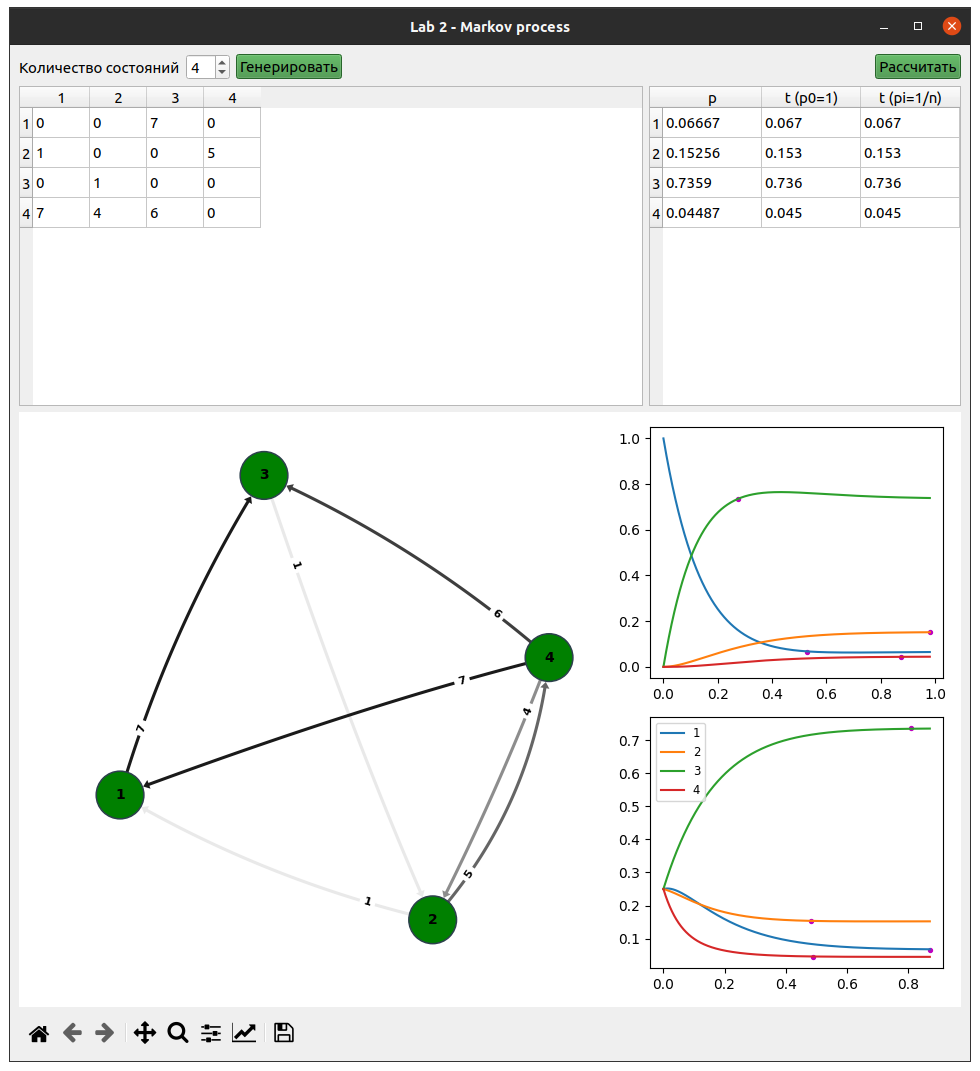
\includegraphics[width=\textwidth]{2/4}
\end{figure}
\begin{figure}[h!]
    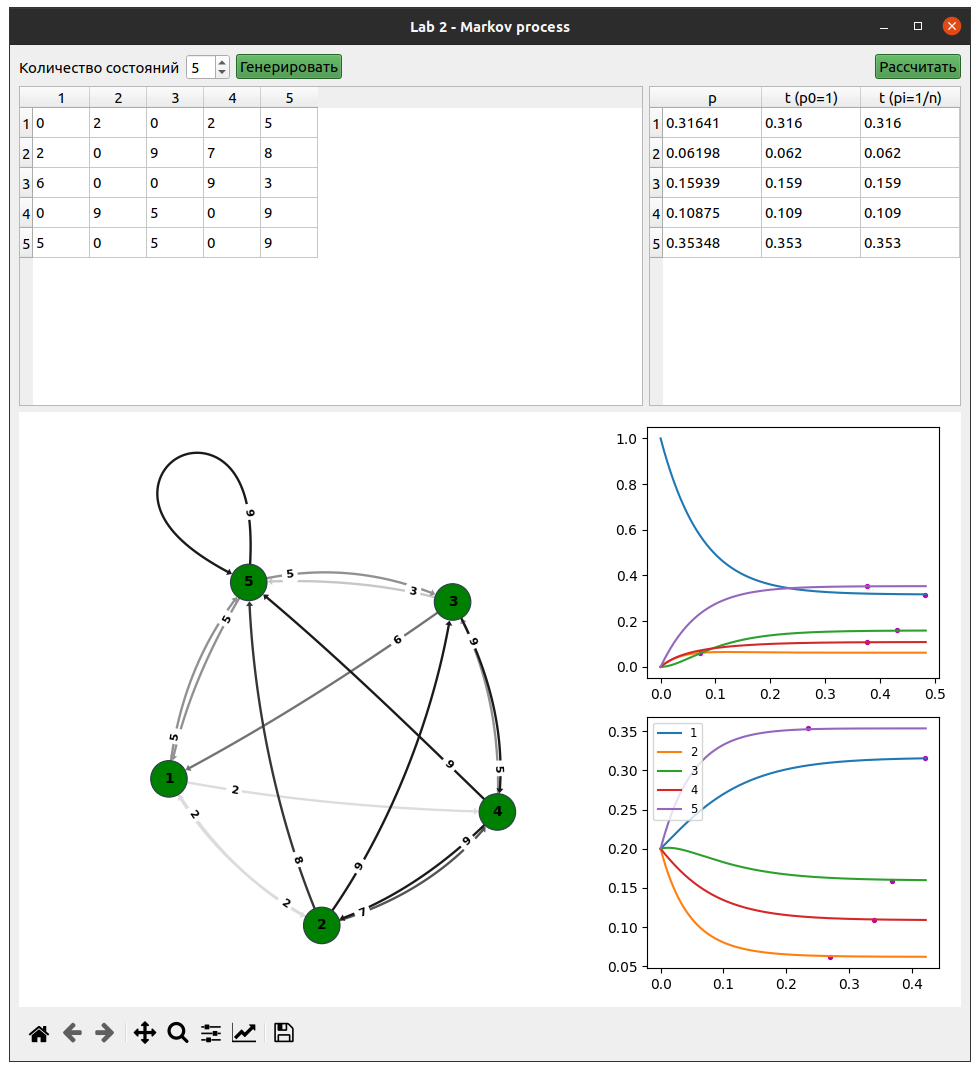
\includegraphics[width=\textwidth]{2/5}
\end{figure}
\begin{figure}[h!]
    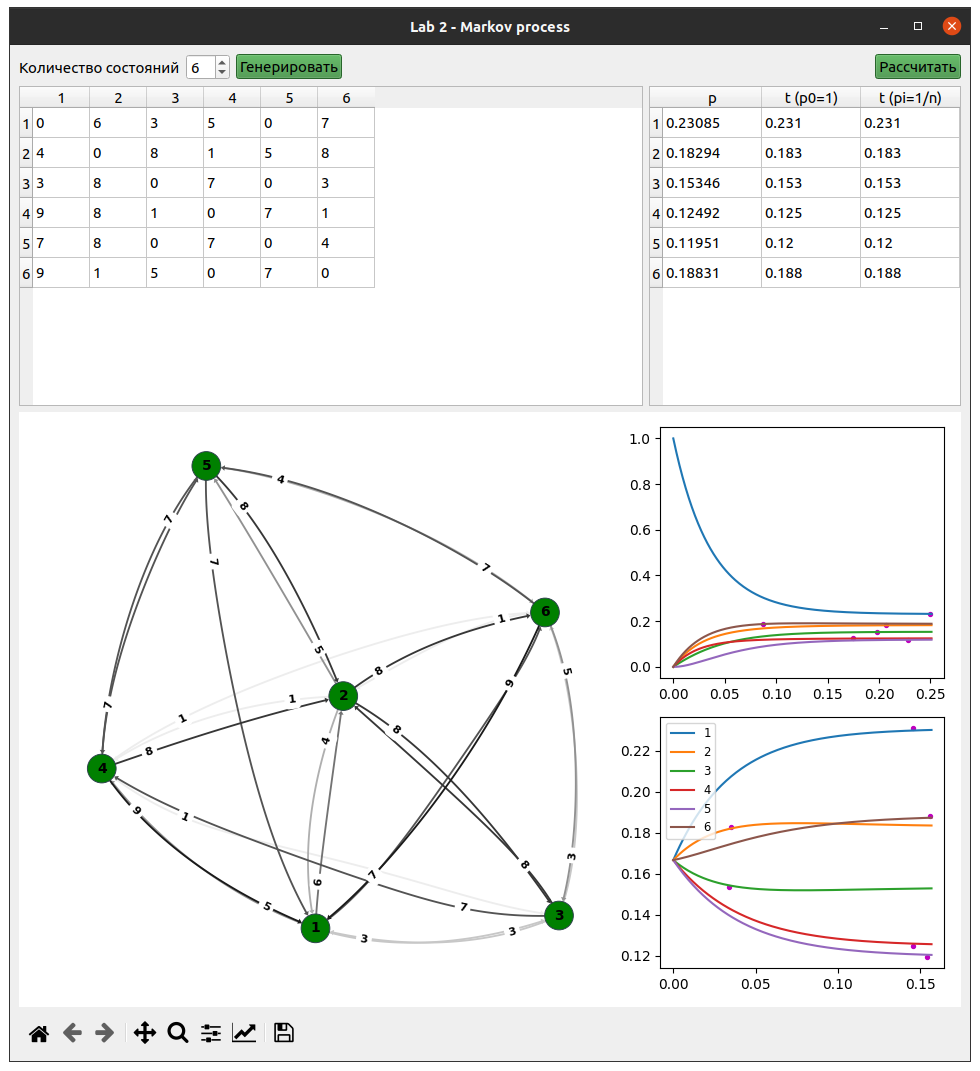
\includegraphics[width=\textwidth]{2/6}
\end{figure}
\begin{figure}[h!]
    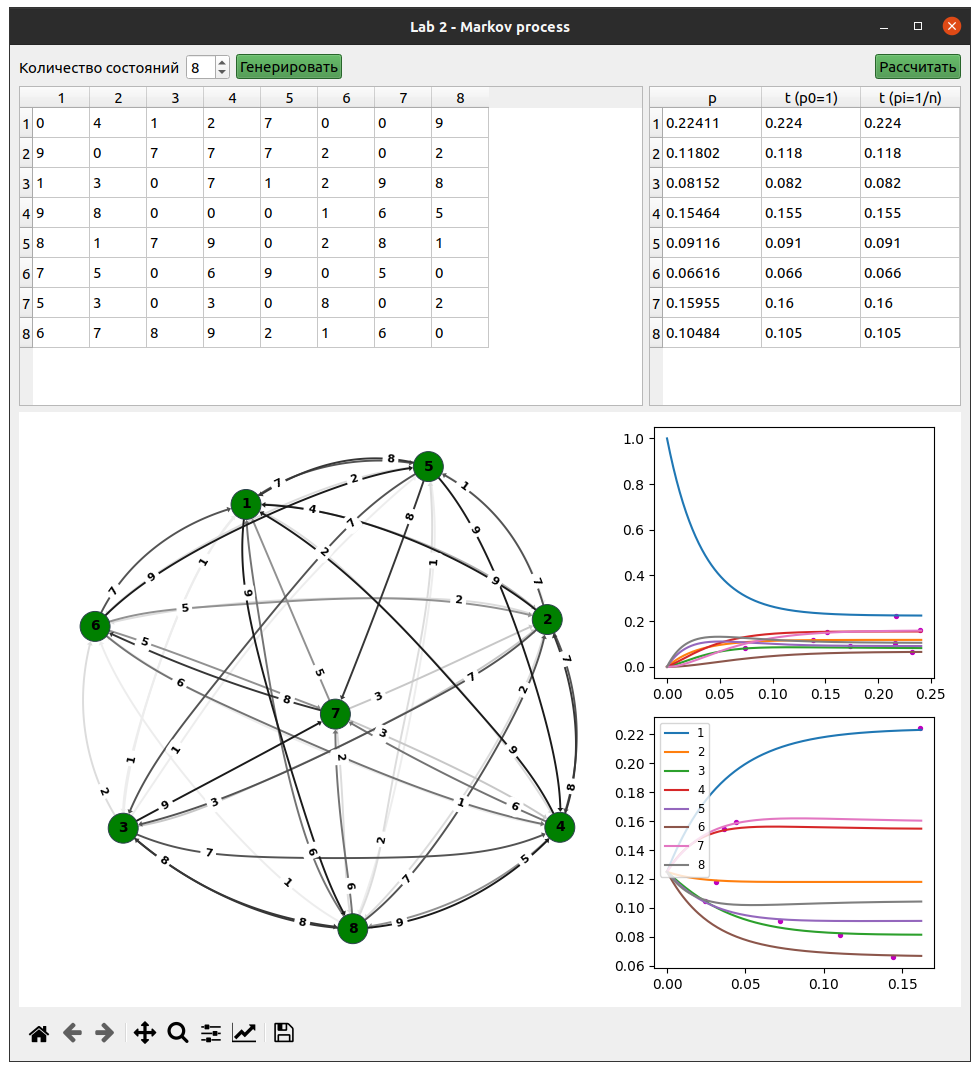
\includegraphics[width=\textwidth]{2/8}
\end{figure}


\clearpage
\section{Листинг кода}

\lstinputlisting[
    language=Python,
    caption=Программная реализация определения времени пребывания сложной системы в каждом из состояний
]{../2/markov.py}
